\section{Regular Expressions}
\subsection{Regular Language}
Strings can be broken down as "regular expressions", a logical expression that can be used to solve matching and searching problems. A matching problem can be checking if a string is a valid password that contains at least $X$ characters and at least $Y$ digits. A searching problem can be, given a string, list all occurrences of an email address in it. Regexps are used to solve problems like these.

For example, the regular expression \textbf{c(bb$|$ca)$^*$} will return true when matched with \textbf{cbbbbca} but return false when matched with \textbf{bca}. To solve problems using regexps, we can use Deterministic Finite Automatons (DFAs). They are deterministic because the initial state and the result of each transition are specified, and finite because there set of states is a finite set. When given a string, in the DFA seen, it will process each letter one at a time, going from state and following the transitions.

\begin{figure}[!htb]
	\center{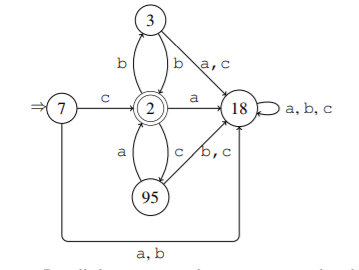
\includegraphics[width=3cm]
		{models/dfa}}
	\caption{\label{fig:dfa} Example of a DFA}
\end{figure}

As you can see, there are a few loops/areas where the DFA will definitely return false once it reaches a certain point. A more efficient way to deal with these things is to completely remove the transitions, and have it return a failure at points we know it will definitely fail. These are called partial DFAs, denoted by the $\delta$ symbol ($\delta$DFA). These are usually faster to write and run faster.

What happens when the DFA is not deterministic? An NFA if you will. NFAs differ from DFAs in two ways.
\begin{itemize}
	\item An NFA can have several initial states
	\item From a given state, when $a$ is input, there can be several possible next states.
\end{itemize}
NFAs are a relation and not a function. They can still return acceptable words, but a program can make no use of it since its, well, non-deterministic. However, there are ways to determinize an NFA. The best, basic way to accomplish this is to combine states into a set of state transitions if they match similar inputs/outputs. Conversion can take a few steps, but it's fairly simple and systematic in this regard.

Some trouble can pop up from NFAs with an $\epsilon$ transition, or an empty transitions. These bad boys can change from one state to another for literally no reason. These NFAs are called $\epsilon$NFAs, which seems obvious. With this out of the way, let's make note of Kleene's Theorem. \textbf{For a language $L$, the following are equivalent:}
\begin{itemize}
	\item L is regular
	\item The matching problem for L can be solved by a DFA.
\end{itemize}

A systematic way to turn a regexp to an equal DFA:
\begin{enumerate}
	\item Convert the regexp into an $\epsilon$NFA
	\item Convert it down to an NFA
	\item Convert it further down to a DFA.
	\item Minimize DFA size by identifying equivalent states, removing unreachable states and just general refactoring.
\end{enumerate}
\subsection{Non-regular Language}
Well Balanced Bracket Example
Grammar / Derivations
Ambiguity
\section{Turing Machines}
\subsection{Turing Machines}
Define
Instruction set
Example
Variants
\section{Complexity}
\subsection{Complexity of Programs}
Important Summations
Big-O
Polynomial Time
Example
\subsection{P and NP}
Search Problem
NP examples
NP = P
\section{Decidability and Completeness}
Define
\subsection{Halting Problem}
Example from lecture, might appear in exam
\subsection{Reduction and Decidability}
P -> Q, Q -> P
Semantics
Rice's Theorem
iF a MeThOd iS bLuE ?
\section{Lambda Calculus}
Notation
$\beta$-reduction and $\alpha$-equivalent
Reduction graph
Example